\documentclass[10pt]{article}
\usepackage[utf8]{inputenc}
\usepackage[T1]{fontenc}
\usepackage{mathptmx}
\usepackage[margin=1.8cm]{geometry}
\usepackage{graphicx,booktabs,xcolor,url,array,tikz,caption,float}
\usetikzlibrary{arrows.meta,positioning}
\newcommand{\pend}[1]{\textcolor{red}{[#1]}}
\renewcommand{\thetable}{S\arabic{table}}
\renewcommand{\thefigure}{S\arabic{figure}}
\captionsetup{font=small}
\title{Supplementary material\\[2pt]\large Gains on Synthetic Occlusion Do Not Anticipate Robustness to Real Occlusion in Person Detection}
\author{Apaza Hilasaca, Condori Quispe, Ramos Quispe (UPeU, Juliaca)}
\date{20 October 2026}
\begin{document}
\maketitle
\noindent Every table in this supplement is generated by \path{shortpaper5/suplemento_tablas.py} from the project's result files (\path{informes/analisis_final/}); no figure is typed by hand. Analyses marked as post hoc were declared after seeing the results and decide no hypothesis.

\section{Objectives, method and evidence}
\begin{table}[H]\centering\small
\caption{Mapping of specific objectives, method, evidence and pending work.}
\begin{tabular}{@{}p{3.3cm}p{4.6cm}p{5.4cm}p{2.6cm}@{}}\toprule
\textbf{Objective} & \textbf{Method} & \textbf{Evidence} & \textbf{Pending} \\\midrule
OE1. Degradation under occlusion & Stratified AP@0.5 with \emph{ignore} regions, three sources & 0.82 (unoccluded) to 0.24 (severe), YOLOv11s on ExDark & --- \\
OE2. Effect of augmentation by occluder & V3 vs.\ V1, control and 3 real sources; patches, silhouettes, diffusion, real geometry and depth & 13 of 13 controls; 4 of 39 real cells, none stable and occlusion-specific; null mean effect with equal exposure (with the four torchvision blocks: 17 of 17 and 6 of 51) & Occlusion mined from real images \\
OE3. Dependence on the detector & YOLOv11s, YOLOv11m, YOLO26s, RT-DETR-l, RetinaNet, Faster R-CNN & Same pattern in the first five; Faster R-CNN transfers with silhouettes on NightOwls and CityPersons (H15 refuted), but not with diffusion or depth (H16a and H16b refuted), and RetinaNet with silhouettes does not transfer (H17) & Another two-stage detector or backbone \\
OE4. Domain and data volume & Retraining on CityPersons (H6, H11); NightOwls from 2,000 to 20,000 images (H7) & The deficit persists; the in-domain gain was not confirmed (H11) & --- \\
OE5. Mechanism & Recall, false positives, confidence; visibility; realism (H13); cross-family matrix & Synthetically occluded people remain distinguishable from real ones; lower recall with higher confidence & Confirmatory test of the mechanism \\
OE6--OE7. Attention module; annotation reliability & FPS and parameters; inter-annotator $\kappa$ & No gain from the module (H1, H2), FPS at 82\,\%; $\kappa$ 0.06--0.60 & Embedded-device test \\
\bottomrule\end{tabular}\end{table}

\noindent\textbf{Variants of the original design.} Experiment 1 had four variants: V1 (baseline), V2 (CBAM attention module in the neck), V3 (occlusion augmentation) and V4 (both). H1 (V4 improves on V1) and H2 (V3 improves more than V2) were not confirmed, and H5 (silhouettes reduce the gap) only partially, because the gap closed by real occlusion getting worse. The attention module cut FPS to 82\,\% (161--184 versus 144--157) with no gain on real occlusion. From iteration 2 on the question is transfer and only V1 and V3 are compared.

\section{Hypotheses and pre-specification}
The global SHA-256 fingerprint of the protocol proves that no frozen file changed after the freeze, but the date is recorded by the project itself (\path{CAMBIOS_PROTOCOLO.md}), not by a third party. The ``first run'' column comes from each run's log and shows that every freeze precedes training. All dates are in 2026.

\begin{table}[H]\centering\scriptsize
\caption{Hypotheses, prediction, freeze and verdict. The fingerprint is that of the frozen protocol (global SHA-256, first 8 characters); the date is self-recorded by the project, not by a third party. First run: start of the first valid run of the block, from its log (local time, UTC$-$5, on the laptop; UTC on RunPod: H11, H12 and H14--H17).}\label{tab:s-hip}
\resizebox{\textwidth}{!}{\begin{tabular}{@{}l p{6.3cm} l l l l p{3.2cm}@{}}\toprule
Hyp. & Prediction & File & Version and fingerprint & Frozen & First run & Verdict \\
\midrule
H1--H3 & V4 and V3 improve occluded AP by $\geq$2 pp over V1 (H1, H2) and the gain transfers to real occlusion (H3) & \texttt{PROTOCOLO.md} & v1.0 \texttt{c5002ea5} & 2026-09-11 08:09 & 2026-09-11 08:47 & Not confirmed (0 of 3 sources in H3) \\
H4, H5 & With silhouettes the gain transfers (H4); smaller synthetic gain and gap (H5) & \texttt{PROTOCOLO\_v2.md} & v2.0 \texttt{9915d90f} & 2026-09-12 12:51 & 2026-09-12 12:54 & H4 not confirmed (0 of 3); H5 partial \\
H6 & No transfer when retraining on CityPersons & \texttt{PREREGISTRO\_H6\_H7.md} & v3.0 \texttt{e971ab8b} & 2026-09-19 16:48 & 2026-09-19 16:48 & Not detected (0 of 3) \\
H7 & No transfer with 20,000 night images & \texttt{PREREGISTRO\_H6\_H7.md} & v3.1 \texttt{b0043c89} & 2026-09-25 20:58 & 2026-09-25 20:59 & Inconclusive (no control) \\
H8 & No transfer with RT-DETR-l & \texttt{PREREGISTRO\_H8.md} & v3.2 \texttt{51c0a2d8} & 2026-09-26 18:52 & 2026-09-26 18:52 & Not detected (0 of 3) \\
H9 & No transfer with diffusion occluders & \texttt{PREREGISTRO\_H9.md} & v3.3b \texttt{243acffb} & 2026-10-03 01:29 & 2026-10-03 01:29 & Not detected (1 of 3) \\
H9b & Same with 30 fixed epochs & \texttt{PREREGISTRO\_H9b.md} & v3.4 \texttt{51786d9d} & 2026-10-06 09:01 & 2026-10-06 09:02 & Not detected (0 of 3) \\
H10 & No transfer with real-occlusion geometry & \texttt{PREREGISTRO\_H10.md} & v3.5 \texttt{1489961a} & 2026-10-06 18:27 & 2026-10-07 05:03 & Not detected (1 of 3) \\
H11 & Gain $\geq$2 pp at CityPersons visibility 0.20--0.50 with equal exposure & \texttt{PREREGISTRO\_H11.md} & v3.6b \texttt{bd2666fd} & 2026-10-13 14:38 & 2026-10-13 20:37 & Not confirmed \\
H12 & No transfer with YOLOv11m (silhouettes, H12a; diffusion, H12b) & \texttt{PREREGISTRO\_H12.md} & v3.7b \texttt{ef6138c1} & 2026-10-13 21:06 & 2026-10-17 14:50 & Not detected (0 of 3 and 0 of 3) \\
H13 & AUC(patches) $>$ AUC(silhouettes) $>$ AUC(diffusion) with DINOv2 & \texttt{PREREGISTRO\_H13.md} & v3.8 \texttt{7ce00c9c} & 2026-10-17 09:48 & no training & Partially confirmed \\
H14 & No transfer with depth order & \texttt{PREREGISTRO\_H14.md} & v3.9 \texttt{264ac449} & 2026-10-17 10:10 & 2026-10-17 16:33 & Not detected (1 of 3) \\
H15 & No transfer with Faster R-CNN & \texttt{PREREGISTRO\_H15.md} & v3.10 \texttt{b7843b3a} & 2026-10-20 16:20 & 2026-10-21 13:31 & Passes the rule (2 of 3) \\
H16a, H16b & With Faster R-CNN transfer also occurs with diffusion (H16a) and depth order (H16b) & \texttt{PREREGISTRO\_H16\_H17.md} & v3.11 \texttt{e9b85aee} & 2026-10-22 07:50 & 2026-10-22 13:57 & Refuted (0 of 3 and 0 of 3) \\
H17 & No transfer with RetinaNet (one-stage, same backbone as H15, its own reference recipe) & \texttt{PREREGISTRO\_H16\_H17.md} & v3.11 \texttt{e9b85aee} & 2026-10-22 07:50 & 2026-10-22 13:08 & Not detected (0 of 3) \\
\bottomrule\end{tabular}}\end{table}


\section{Run log and recipes}
The 104 valid runs are: 14 in experiment 1 (12 of V1--V4 and two controls, without occlusion augmentation and without pre-training), 12 in iteration 2 (V1--V4), 6 with YOLO26s, 6 in H6, 12 in H7 (two per rung of 2,000, 5,000 and 10,000 with seed 0, and six at 20,000), 6 in H8 and 3 in H9 (its V1 is that of iteration 2): 59 in the first seven blocks; then 6 in H9b, 6 in H10 (its V1 is that of H9b), 6 in H11, 9 in H12, 6 in the seed extension, 6 in H14, 6 in H15, 6 in H16 (V3 with diffusion and with depth; its V1 is that of H15), 6 in H17 and 1 replicate of the H15 V1 seed 0 on another machine: 117 in total. Versions: Ultralytics 8.4.143; PyTorch 2.11 with CUDA 12.8 on the laptop and 2.8 with CUDA 12.8 on RunPod; torchvision 0.23 for Faster R-CNN and RetinaNet. The V1 replicate differs from the original by $-0.87$ (NightOwls), $-1.92$ (CityPersons) and $+3.42$ pp (ExDark, 101 instances), above the 2 pp threshold declared in the pre-registration: the variation between machines is of the order of the H15 gains.

\begin{table}[H]\centering\scriptsize
\caption{Run log by block (per-run detail in \texttt{informes/analisis\_final/registro\_corridas.csv}). Epochs: trained and of the evaluated weights, min--max. With validation selection, the evaluated epoch is the one with maximum validation mAP50-95 (ExDark val and occluded val).}\label{tab:s-registro}
\resizebox{\textwidth}{!}{\begin{tabular}{@{}l l r l l l l r@{}}\toprule
Block & Detector & Runs & V1 ep. (eval./train.) & V3 ep. (eval./train.) & Exposure rule & Machine & Hours \\
\midrule
Exp. 1 (parches) & YOLOv11s, YOLOv11s+CBAM & 14 & 2 / 22--40 & 2 / 22 & validation selection & RTX 5050 Laptop & 7.8 \\
Iteración 2 (siluetas) & YOLOv11s, YOLOv11s+CBAM & 12 & 1--2 / 21--22 & 37--89 / 57--100 & validation selection & RTX 5050 Laptop & 10.0 \\
Réplica YOLO26s & YOLO26s & 6 & 1--3 / 21--23 & 82--87 / 100 & validation selection & RTX 5050 Laptop & 8.2 \\
H6 (CityPersons) & YOLOv11s & 6 & 38--51 / 58--71 & 85--88 / 100 & validation selection & RTX 5050 Laptop & 18.4 \\
H7 peldaño 2 000 & YOLOv11s & 2 & 2 / 22 & 43 / 63 & fixed presentations, patience 1/5 & RTX 5050 Laptop & 2.5 \\
H7 peldaño 5 000 & YOLOv11s & 2 & 1 / 9 & 35 / 40 & fixed presentations, patience 1/5 & RTX 5050 Laptop & 3.5 \\
H7 peldaño 10 000 & YOLOv11s & 2 & 2 / 6 & 20 / 20 & fixed presentations, patience 1/5 & RTX 5050 Laptop & 3.7 \\
H7 peldaño 20 000 & YOLOv11s & 6 & 1--2 / 3--4 & 2--9 / 4--10 & fixed presentations, patience 1/5 & RTX 5050 Laptop & 9.0 \\
H8 (RT-DETR-l) & RT-DETR-l & 6 & --- & --- & validation selection & RTX 5050 Laptop & 15.0 \\
H9 (generativa) & YOLOv11s & 3 & --- & 1--2 / 21--22 & validation selection & RTX 5050 Laptop & 1.2 \\
H9b (generativa, 30 ep.) & YOLOv11s & 6 & 30 / 30 & 30 / 30 & 30 fixed epochs & RTX 5050 Laptop & 3.5 \\
H10 (geometría, 30 ep.) & YOLOv11s & 3 & --- & 30 / 30 & 30 fixed epochs & RTX 5050 Laptop & 1.9 \\
H10-s (siluetas, 30 ep.) & YOLOv11s & 3 & --- & 30 / 30 & 30 fixed epochs & RTX 5050 Laptop & 1.8 \\
H11 (CityPersons, 60 ep.) & YOLOv11s & 6 & 60 / 60 & 60 / 60 & 60 fixed epochs & RTX 4090 & 1.9 \\
H12 (YOLOv11m) & YOLOv11m & 9 & 30 / 30 & 30 / 30 & 30 fixed epochs & RTX 4090 & 1.0 \\
Extensión de semillas & YOLOv11s & 6 & 30 / 30 & 30 / 30 & 30 fixed epochs & RTX 4090 & 0.5 \\
H14 (profundidad, 30 ep.) & YOLOv11s & 6 & 30 / 30 & 30 / 30 & 30 fixed epochs & RTX 4090 & 0.5 \\
H15 (Faster R-CNN, 30 ep.) & Faster R-CNN R50-FPN v2 & 6 & 30 / 30 & 30 / 30 & 30 fixed epochs & RTX 4090 & 2.6 \\
H16a (Faster R-CNN, generativa) & Faster R-CNN R50-FPN v2 & 3 & --- & 30 / 30 & 30 fixed epochs & RTX 4090 & 1.9 \\
H16b (Faster R-CNN, profundidad) & Faster R-CNN R50-FPN v2 & 3 & --- & 30 / 30 & 30 fixed epochs & RTX 4090 & 1.9 \\
H17 (RetinaNet, 30 ep.) & RetinaNet R50-FPN v2 & 6 & 30 / 30 & 30 / 30 & 30 fixed epochs & RTX 4090 & 2.5 \\
Réplica de V1 entre pods & Faster R-CNN R50-FPN v2 & 1 & 30 / 30 & --- & 30 fixed epochs & RTX 4090 & 0.2 \\
\midrule Total & & 117 & & & & & 99.3 \\
\bottomrule\end{tabular}}\end{table}


\begin{table}[H]\centering\small
\caption{Training recipe by detector. The base augmentation (identical in V1 and V3) uses the Ultralytics 8.4 values fixed in \texttt{config/aumento\_base.yaml}: HSV (0.015, 0.7, 0.4), translation 0.1, scale 0.5, horizontal flip 0.5, mosaic 1.0 with no mosaic in the last 10 epochs.}
\begin{tabular}{@{}p{2.6cm}p{2.2cm}p{2.6cm}p{1.9cm}p{1.6cm}p{1.6cm}p{2.6cm}@{}}\toprule
Detector & Optimizer & LR (final) & Warm-up & Weight decay & Batch & Epochs \\\midrule
YOLOv11s/m, YOLO26s & SGD, momentum 0.937 & 0.002 (linear to 1\,\%) & 3 epochs & $5\cdot10^{-4}$ & 16 & up to 100 (pat. 20) or 30/60 fixed \\
RT-DETR-l & AdamW, $\beta_1$ 0.9 & $10^{-4}$ (linear to 1\,\%) & 3 epochs, bias 0 & $10^{-4}$ & 8 (acc.\ to 64) & up to 100 (pat. 20) \\
Faster R-CNN R50-FPN v2 & SGD, momentum 0.9 & 0.01, $\times$0.1 at 20 and 27 & 500 iterations & $10^{-4}$ & 8 & 30 fixed \\
RetinaNet R50-FPN v2 & SGD, momentum 0.9 & 0.005, $\times$0.1 at 20 and 27 & 500 iterations & $10^{-4}$ & 8 & 30 fixed \\
\bottomrule\end{tabular}\end{table}

\section{Augmentation and control of each family}
\begin{table}[H]\centering\small
\caption{Augmentation (training) and control (test) parameters. The control always uses the 841 ExDark test images and all their valid people, with coverage 0.70--1.00, and occluders the model did not see in training.}
\begin{tabular}{@{}p{2.2cm}p{7.0cm}p{6.6cm}@{}}\toprule
Family & Training (V3) & Control \\\midrule
Patches & Texture rectangles (0.4), object cut-outs (0.5) or opaque (0.1); $p=0.5$ per image, 1--3 people, coverage 0.30--0.85; \emph{train} cut-out bank & \texttt{opaco\_severa}: opaque border band; \emph{test} cut-out bank, disjoint from \emph{train} \\
Silhouettes & Masked silhouettes of real objects and people (person with prob.\ 0.5), luminance matching; same $p$, number and coverage; \texttt{siluetas\_train} bank & \texttt{silueta\_severa}: \texttt{siluetas\_test} bank (disjoint images) \\
Diffusion & Stable Diffusion 1.5 inpainting, 20 steps, guidance 7.5, ten COCO objects (``a parked car'', ``a bicycle''\ldots) with the suffix ``at night, low light, realistic photo''; two versions per image generated in advance and substituted with $p=0.15$ (with mosaic) or 0.5 (without); quality check with YOLOv11s-seg (rejected if $>$30\,\% of the mask is still a person) & \texttt{generativa\_severa}: same prompts and model, generated anew on the test images with other seeds (96.2\,\% accepted) \\
Real geometry & Silhouettes placed over the hidden region of real CityPersons \emph{train} visibility patterns, coverage 0.40--0.95 & \texttt{geometria\_severa}: internal-validation patterns and \emph{test} bank (mean IoU cut-out--hidden region 0.61) \\
Depth order & Object cut-outs standing on the ground in front of the person and composited only where the scene is farther (Depth Anything V2 Small); 2 versions per image, same substitution as diffusion & \texttt{profundidad\_severa}: \texttt{siluetas\_test} bank \\
\bottomrule\end{tabular}\end{table}

\begin{figure}[H]\centering
\includegraphics[width=0.92\textwidth]{fig_cualitativa.png}
\caption{Top: annotated real occlusion in the three sources (orange box: evaluated person). Bottom: the same ExDark test person in each synthetic family's control (green box).}
\end{figure}

\begin{figure}[H]\centering
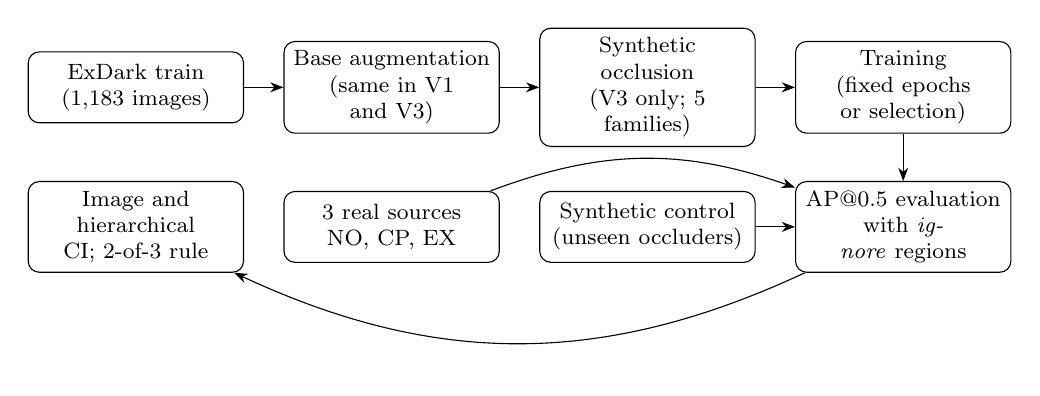
\begin{tikzpicture}[n/.style={draw,rounded corners,align=center,font=\footnotesize,minimum height=0.9cm,text width=2.5cm},a/.style={-Stealth}]
\node[n] (d) {ExDark train\\(1,183 images)};
\node[n,right=0.5cm of d] (b) {Base augmentation\\(same in V1 and V3)};
\node[n,right=0.5cm of b] (o) {Synthetic occlusion\\(V3 only; 5 families)};
\node[n,right=0.5cm of o] (t) {Training\\(fixed epochs or selection)};
\node[n,below=0.6cm of t] (e) {AP@0.5 evaluation\\with \emph{ignore} regions};
\node[n,left=0.5cm of e] (c) {Synthetic control\\(unseen occluders)};
\node[n,left=0.5cm of c] (r) {3 real sources\\NO, CP, EX};
\node[n,left=0.5cm of r] (v) {Image and hierarchical CI; 2-of-3 rule};
\draw[a] (d)--(b); \draw[a] (b)--(o); \draw[a] (o)--(t); \draw[a] (t)--(e); \draw[a] (c)--(e); \draw[a] (r) to[bend left=20] (e); \draw[a] (e) to[bend left=25] (v);
\end{tikzpicture}
\caption{Pipeline of each block. Occlusion is applied to the RGB image after base augmentation and before formatting, in training only; validation and test are never occluded except in the control.}
\end{figure}

\section{All cells and statistical analysis}
\begin{table}[H]\centering\scriptsize
\caption{All cells: V3$-$V1 in AP@0.5 (pp), 95\,\% CI over images (1,000 replicates) and hierarchical (seeds and images, 2,000), 3 seeds per variant. * passes: estimate $\geq+2$ and image CI $>0$. $\dagger$ rules out a $+2$ pp gain (upper image-CI limit $<+2$). Exposure: equal (fixed epochs), unequal (V1 and V3 selected at different epochs by validation) or early (both at epochs 1--2).}\label{tab:s-celdas}
\resizebox{\textwidth}{!}{\begin{tabular}{@{}l l l r l l | l r l l@{}}\toprule
Block & Exp. & Cell & $\Delta$ & Image CI & Hierarchical CI & Cell & $\Delta$ & Image CI & Hierarchical CI \\
\midrule
H3 & early & Control & +60.92* & [+58.50; +63.41] & [+56.75; +64.95] & NO & $-$3.17$^\dagger$ & [$-$4.58; $-$1.74] & [$-$7.94; +2.10] \\
 & & CP & $-$0.36$^\dagger$ & [$-$1.06; +0.31] & [$-$2.42; +1.62] & EX & $-$3.25$^\dagger$ & [$-$5.81; $-$0.21] & [$-$7.11; +0.89] \\
H4 & unequal & Control & +10.63* & [+9.42; +12.15] & [+8.95; +12.50] & NO & $-$16.79$^\dagger$ & [$-$19.59; $-$13.96] & [$-$20.41; $-$12.96] \\
 & & CP & $-$3.94$^\dagger$ & [$-$5.66; $-$2.41] & [$-$7.14; $-$1.02] & EX & $-$5.02$^\dagger$ & [$-$10.72; +0.50] & [$-$11.89; +1.28] \\
H4-Y26 & unequal & Control & +12.01* & [+10.61; +13.57] & [+10.32; +13.79] & NO & $-$14.31$^\dagger$ & [$-$17.35; $-$11.10] & [$-$18.07; $-$10.14] \\
 & & CP & $-$4.42$^\dagger$ & [$-$5.95; $-$2.63] & [$-$6.89; $-$1.65] & EX & $-$3.51$^\dagger$ & [$-$8.38; +1.21] & [$-$9.48; +1.86] \\
H6 & unequal & Control & +23.74* & [+21.09; +26.51] & [+20.44; +27.22] & NO & $-$1.35$^\dagger$ & [$-$2.85; +0.20] & [$-$3.47; +0.68] \\
 & & CP & +1.82 & [+0.31; +3.31] & [$-$0.86; +4.42] & EX & +0.94 & [$-$2.53; +4.72] & [$-$4.06; +6.68] \\
H7 & unequal & NO & $-$1.43$^\dagger$ & [$-$3.98; +1.00] & [$-$4.45; +1.56] & CP & $-$3.94$^\dagger$ & [$-$5.62; $-$2.27] & [$-$8.15; +0.78] \\
 & & EX & $-$9.15$^\dagger$ & [$-$13.94; $-$5.66] & [$-$17.22; $-$3.26] & & & & \\
H8 & unequal & Control & +10.97* & [+9.57; +12.36] & [+9.32; +12.83] & NO & $-$6.98$^\dagger$ & [$-$8.95; $-$5.11] & [$-$11.16; $-$2.81] \\
 & & CP & $-$3.47$^\dagger$ & [$-$4.86; $-$1.81] & [$-$6.27; $-$0.74] & EX & $-$2.21$^\dagger$ & [$-$6.16; +1.59] & [$-$7.61; +3.39] \\
H9 & early & Control & +2.60* & [+2.12; +3.09] & [+0.25; +4.33] & NO & $-$1.93$^\dagger$ & [$-$2.89; $-$0.88] & [$-$3.87; $-$0.12] \\
 & & CP & +1.23 & [+0.36; +2.11] & [$-$1.70; +4.03] & EX & +2.82* & [+0.37; +5.99] & [$-$1.23; +7.40] \\
H9b & equal & Control & +15.23* & [+14.00; +17.16] & [+13.81; +17.45] & NO & +0.01$^\dagger$ & [$-$1.02; +1.20] & [$-$1.60; +1.82] \\
 & & CP & +1.52 & [+0.79; +2.66] & [$-$0.02; +3.39] & EX & $-$3.03$^\dagger$ & [$-$6.77; +0.99] & [$-$8.85; +2.89] \\
H11 & equal & Control & +24.66* & [+21.62; +27.47] & [+21.44; +28.09] & NO & +1.95 & [+0.93; +3.21] & [$-$0.16; +4.66] \\
 & & CP & +1.31 & [$-$0.28; +2.78] & [$-$0.85; +3.46] & EX & $-$2.44 & [$-$6.77; +2.36] & [$-$7.34; +3.23] \\
H10 & equal & Control & +18.39* & [+15.61; +21.30] & [+15.57; +21.47] & NO & $-$2.05$^\dagger$ & [$-$3.26; $-$0.92] & [$-$4.62; +0.29] \\
 & & CP & +2.37* & [+1.52; +3.52] & [+0.63; +4.61] & EX & $-$4.88$^\dagger$ & [$-$9.08; $-$0.82] & [$-$11.58; +1.03] \\
H10-s & equal & Control & +10.99* & [+9.62; +12.62] & [+9.58; +12.68] & NO & $-$1.12$^\dagger$ & [$-$2.13; +0.08] & [$-$2.58; +0.49] \\
 & & CP & +2.26* & [+1.44; +3.47] & [+0.72; +4.04] & EX & $-$3.50$^\dagger$ & [$-$7.64; +0.08] & [$-$9.63; +1.86] \\
H12a & equal & Control & +14.45* & [+12.76; +16.37] & [+12.67; +16.46] & NO & $-$0.39$^\dagger$ & [$-$1.55; +0.89] & [$-$3.92; +2.77] \\
 & & CP & +0.25$^\dagger$ & [$-$0.63; +1.27] & [$-$1.32; +2.12] & EX & +3.04 & [$-$1.07; +6.63] & [$-$2.63; +8.31] \\
H12b & equal & Control & +19.04* & [+17.49; +21.03] & [+17.35; +21.21] & NO & +0.78 & [$-$0.42; +2.16] & [$-$3.21; +4.28] \\
 & & CP & +1.11 & [+0.14; +2.16] & [$-$0.47; +2.89] & EX & $-$0.56 & [$-$4.07; +3.19] & [$-$5.77; +5.06] \\
H14 & equal & Control & +7.42* & [+6.40; +8.79] & [+6.13; +9.13] & NO & $-$1.50$^\dagger$ & [$-$2.75; $-$0.37] & [$-$3.40; +0.26] \\
 & & CP & $-$0.16$^\dagger$ & [$-$1.21; +0.75] & [$-$1.85; +1.31] & EX & +5.49* & [+1.63; +9.30] & [$-$0.35; +11.14] \\
H15 & equal & Control & +14.72* & [+13.04; +16.66] & [+12.97; +16.63] & NO & +3.28* & [+1.64; +4.79] & [+0.67; +5.81] \\
 & & CP & +2.33* & [+1.01; +3.69] & [+0.13; +4.92] & EX & $-$1.00 & [$-$5.61; +3.24] & [$-$6.71; +4.04] \\
\bottomrule\end{tabular}}\end{table}


\begin{figure}[H]\centering
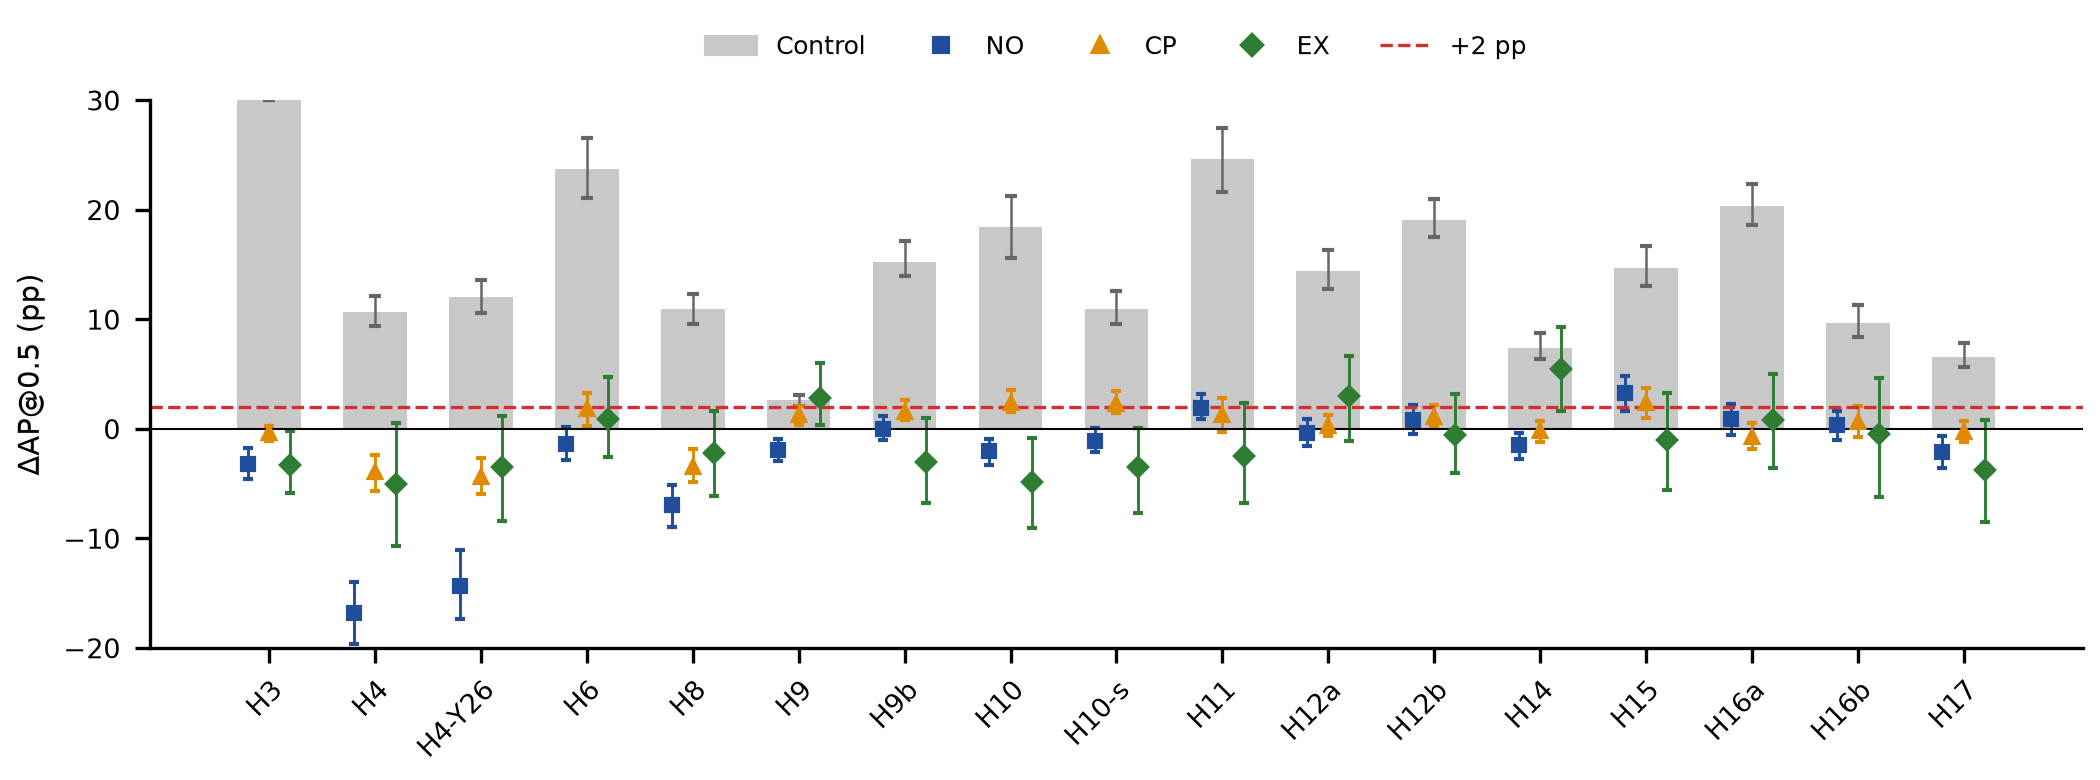
\includegraphics[width=\textwidth]{fig_gap_ic.png}
\caption{Synthetic control (bars) and real sources (markers) per block, with 95\,\% image CIs. The H3 bar is cut at +30 (+60.9).}
\end{figure}

\begin{table}[H]\centering\scriptsize
\caption{Counts and declared (post hoc) statistical analyses: 13 blocks with a control, 39 real cells. Mixed model: real gain $\sim$ synthetic gain (standardized) + source, with a random intercept per block.}\label{tab:s-estad}
\begin{tabular}{@{}p{5.0cm} p{2.9cm}@{}}\toprule
Real cells that pass (estimate $\geq+2$ and CI $>0$) & 4 of 39 (hierarchical CI: 2) \\
Rule out a +2 pp gain (non-superiority, one-sided 2.5 \%) & 24 of 39 (hierarchical: 19) \\
Equal exposure (21 cells): pass / negative with CI / mean & 3 / 3 / +0.02 pp \\
Unequal exposure (12 cells): pass / negative with CI / mean & 0 / 6 / $-$4.94 pp \\
Early selection in both (6 cells): pass / negative with CI / mean & 1 / 3 / $-$0.78 pp \\
Without the ExDark proxy: passing cells; blocks with 2 of 2 & 2 of 26; 0 \\
Between-seed SD of V1 AP@0.5 on real sources (median; max.) & 1.53; 4.10 pp (26 groups) \\
Spearman $\rho$, NO (block-bootstrap CI) & +0.41 [$-$0.18; +0.85] \\
Spearman $\rho$, CP (block-bootstrap CI) & +0.30 [$-$0.26; +0.71] \\
Spearman $\rho$, EX (block-bootstrap CI) & $-$0.15 [$-$0.67; +0.54] \\
Mixed model: slope per SD of synthetic gain (14.0 pp) & +0.11 pp [$-$1.74; +1.95], $p=0.91$ \\
Same without H3 & +0.66 pp [$-$1.31; +2.64], $p=0.51$ \\
\bottomrule\end{tabular}\end{table}


\section{Cross-family control matrix}
If the control measured only memory of the specific occluder, a model would gain on its own control and not on those of other families. Table~\ref{tab:s-cruzada} evaluates every family on every control. 13 of the 20 off-diagonal cells pass (also 13 with the hierarchical CI): augmentation transfers from one synthetic occlusion to another, but not to real occlusion (4 of 39). Only the experiment-1 patches stay close to their own control.

\begin{table}[H]\centering\scriptsize
\caption{Cross-family control matrix: V3$-$V1 (AP@0.5, pp, 3 seeds) of each training family (rows) on each family's severe control (columns), image CI in brackets. All controls use ExDark test images and occluder instances unseen in training. Patches: experiment-1 models (epochs 1--2); the rest, 30 fixed epochs.}\label{tab:s-cruzada}
\setlength{\tabcolsep}{2pt}\begin{tabular}{@{}l ccccc@{}}\toprule
Trained with & Patches & Silhouettes & Generative & Real geometry & Depth order \\ \midrule
Patches & \textbf{+60.9} & +1.3 & +3.0 & +0.9 & +0.8 \\
 & {\tiny [+58.52; +63.35]} & {\tiny [+0.79; +1.86]} & {\tiny [+2.54; +3.71]} & {\tiny [+0.15; +1.75]} & {\tiny [+0.49; +1.21]} \\[2pt]
Silhouettes & +18.1 & \textbf{+11.0} & +2.3 & +15.8 & +4.3 \\
 & {\tiny [+16.56; +19.99]} & {\tiny [+9.63; +12.57]} & {\tiny [+1.84; +3.14]} & {\tiny [+13.48; +18.61]} & {\tiny [+3.55; +5.07]} \\[2pt]
Generative & +7.6 & +0.4 & \textbf{+15.2} & +1.9 & +0.7 \\
 & {\tiny [+6.71; +8.63]} & {\tiny [+0.02; +0.87]} & {\tiny [+14.01; +17.20]} & {\tiny [+0.97; +2.97]} & {\tiny [+0.31; +1.05]} \\[2pt]
Real geometry & +13.7 & +6.3 & +1.7 & \textbf{+18.4} & +2.2 \\
 & {\tiny [+12.37; +15.26]} & {\tiny [+5.19; +7.48]} & {\tiny [+1.28; +2.55]} & {\tiny [+15.77; +21.26]} & {\tiny [+1.64; +2.79]} \\[2pt]
Depth order & +8.3 & +6.7 & +3.1 & +11.7 & \textbf{+7.4} \\
 & {\tiny [+7.32; +9.60]} & {\tiny [+5.66; +7.95]} & {\tiny [+2.40; +3.72]} & {\tiny [+9.67; +14.52]} & {\tiny [+6.35; +8.79]} \\[2pt]
\bottomrule\end{tabular}\end{table}


\section{Secondary analyses}
\begin{table}[H]\centering\scriptsize
\caption{Declared secondary analyses: five seeds (YOLOv11s, 30 epochs), the H7 NightOwls ladder (seed 0, NightOwls occluded) and miss rate MR$^{-2}$ (pp; negative = augmentation misses fewer people).}\label{tab:s-extra}
\setlength{\tabcolsep}{2.5pt}\begin{tabular}{@{}l l r l@{}}\toprule
Analysis & Cell & $\Delta$ & CI (images / hierarchical) \\
\midrule
H9b, 5 seeds & NO & $-$0.45 & [$-$1.28; +0.60] / [$-$1.99; +1.23] \\
H9b, 5 seeds & CP & +0.22 & [$-$0.37; +1.02] / [$-$1.39; +2.00] \\
H9b, 5 seeds & EX & $-$1.75 & [$-$4.79; +1.83] / [$-$6.80; +3.46] \\
H10-s, 5 seeds & NO & $-$1.06 & [$-$1.89; $-$0.03] / [$-$2.36; +0.39] \\
H10-s, 5 seeds & CP & +2.06 & [+1.40; +2.99] / [+0.26; +4.17] \\
H10-s, 5 seeds & EX & $-$2.06 & [$-$5.37; +0.97] / [$-$7.27; +2.65] \\
\midrule
H7, 2000 img. & NO & +0.66 & [$-$3.31; +5.13] \\
H7, 5000 img. & NO & $-$1.12 & [$-$4.99; +3.10] \\
H7, 10000 img. & NO & +4.38 & [+0.17; +8.06] \\
H7, 20000 img. & NO & $-$1.43 & [$-$3.98; +1.00] \\
\midrule
MR$^{-2}$ H3 & \multicolumn{3}{l}{NO +2.9; CP $-$0.0; EX +2.4} \\
MR$^{-2}$ H4 & \multicolumn{3}{l}{NO +13.4; CP +1.6; EX +8.2} \\
MR$^{-2}$ H4-Y26 & \multicolumn{3}{l}{NO +10.3; CP +1.6; EX +3.4} \\
MR$^{-2}$ H6 & \multicolumn{3}{l}{NO +2.1; CP $-$3.2; EX +0.2 (1 improve $\geq$2 with CI)} \\
MR$^{-2}$ H7 & \multicolumn{3}{l}{NO +1.4; CP +2.4; EX +14.7} \\
MR$^{-2}$ H8 & \multicolumn{3}{l}{NO +6.3; CP +2.1; EX +2.8} \\
MR$^{-2}$ H9 & \multicolumn{3}{l}{NO +1.4; CP $-$0.9; EX $-$3.2 (1 improve $\geq$2 with CI)} \\
MR$^{-2}$ H9b & \multicolumn{3}{l}{NO $-$0.2; CP $-$1.2; EX +2.9} \\
MR$^{-2}$ H10 & \multicolumn{3}{l}{NO +1.7; CP $-$1.5; EX +4.1} \\
MR$^{-2}$ H10-s & \multicolumn{3}{l}{NO +0.8; CP $-$1.5; EX +3.0} \\
MR$^{-2}$ H11 & \multicolumn{3}{l}{NO $-$1.8; CP $-$0.6; EX +1.1} \\
MR$^{-2}$ H12a & \multicolumn{3}{l}{NO +0.5; CP +0.0; EX $-$4.0 (1 improve $\geq$2 with CI)} \\
MR$^{-2}$ H12b & \multicolumn{3}{l}{NO +0.3; CP $-$0.5; EX +0.6} \\
MR$^{-2}$ H14 & \multicolumn{3}{l}{NO +0.9; CP +0.5; EX $-$3.4 (1 improve $\geq$2 with CI)} \\
MR$^{-2}$ H15 & \multicolumn{3}{l}{NO $-$2.0; CP $-$1.4; EX $-$1.3} \\
\bottomrule\end{tabular}\end{table}


\begin{table}[H]\centering\scriptsize
\caption{CityPersons by annotated visibility (declared post hoc analysis): V3$-$V1 in AP@0.5 (pp) per bin; other people are \emph{ignore} regions.}\label{tab:s-vis}
\setlength{\tabcolsep}{2.5pt}\begin{tabular}{@{}l rrrrrr@{}}\toprule
Block & 0.20--0.35 & 0.35--0.50 & 0.50--0.65 & 0.65--0.80 & 0.80--0.90 & 0.90--1.00 \\ \midrule
H3 & $-$0.1 & +0.4 & +0.3 & +1.2 & +1.1 & +1.7 \\
H4 & $-$0.1 & $-$1.8 & $-$5.4 & $-$9.7 & $-$13.8 & $-$11.9 \\
H4-Y26 & $-$0.3 & $-$1.9 & $-$5.8 & $-$8.5 & $-$12.8 & $-$9.9 \\
H6 & +4.3 & +3.4 & +2.1 & +0.4 & +0.8 & +0.4 \\
H7 & +0.3 & $-$1.3 & $-$8.1 & $-$14.1 & $-$16.4 & $-$15.6 \\
H8 & $-$0.1 & $-$2.5 & $-$6.3 & $-$9.2 & $-$9.8 & $-$7.2 \\
H9 & +0.3 & +1.0 & +1.0 & +2.5 & +3.0 & +2.1 \\
H9b & +0.0 & +0.8 & +2.6 & +3.9 & +5.9 & +5.2 \\
\bottomrule\end{tabular}\end{table}


\noindent\textbf{Realism (H13).} Mean coverage achieved: patches 0.56, silhouettes 0.54, geometry 0.47 and diffusion 0.32 (the quality check left 146 of 400 people unoccluded), against 0.55 for real occlusion. CityPersons has no real occluder masks (only the visible and full boxes), so the IoU between synthetic and real masks cannot be computed; the real-geometry family reproduces the hidden region of real patterns by construction (mean IoU 0.61 between cut-out and hidden region) and does not transfer either (H10).

\noindent\textbf{KID on the occluder region (post hoc).} With DINOv2 on the occluded part only (real: strip of the full box outside the annotated visible box; synthetic: rectangle of the pixels that change with respect to the same unoccluded person), the distance to real occluders is 2.56 [2.08; 3.17] for patches, 3.39 [2.63; 4.23] for silhouettes, 2.75 [1.91; 3.51] for geometry and 2.50 [1.87; 3.02] for diffusion (248 regions; the quality check left 152 unoccluded), against 3.63 [2.77; 4.34] for the same region without an occluder and 0.01 [$-$0.08; 0.10] between two halves of real occluders. Synthetic occluders are somewhat closer to real occluders than an unoccluded region, but none comes close (\path{informes/kid_oclusor.py}).

\section{Literature search}
Three Scopus searches exported on 13 Oct 2026: main equation (A and B, plus at least one of C, D or E; 155 records), two complementary equations (8) and synthetic versus real occlusion without restricting to people (71). They yielded the five seed articles (PRNet++, WALT, MLFFCSP, CamPed and the YOLOX with domain transfer); the search was supported by Scopus AI and Claude, and the authors made the selection by reading the articles. Exact strings, copied from the Scopus search history:

\noindent\textbf{Main equation (155 records)}\\
{\ttfamily\footnotesize\raggedright TITLE-ABS-KEY ( ( ( pedestrian* or person or persons or people or human or humans ) W/4 detect* ) AND ( occlu* OR "partially visible" OR "partial visibility" OR "crowded scene" ) AND ( ( occlu* W/5 ( augment* or synthetic* or simulat* or artificial* or generat* or inpaint* or diffusion or paste or pasted or pasting or erasing ) ) OR "random erasing" OR cutout OR "copy paste" OR "low light" OR "low illumination" OR "poor illumination" OR "poor lighting" OR "dim light" OR "dark scene" OR "dark environment" OR "dark image" OR darkness OR night* OR nocturnal OR exdark OR nightowls OR "cross-dataset" OR "cross-domain" OR "domain gap" OR "domain shift" OR "dataset bias" OR "domain generali{?}ation" OR "out-of-distribution" OR "sim-to-real" OR "synthetic-to-real" OR "real occlusion" OR "natural occlusion" OR "real-world occlusion" OR ( generali{?}ation W/5 ( dataset* or domain* ) ) ) ) AND PUBYEAR > 2021 AND PUBYEAR < 2027 AND ( DOCTYPE ( ar ) OR DOCTYPE ( cp ) OR DOCTYPE ( re ) ) AND LANGUAGE ( english ) AND ( subjarea ( COMP ) OR subjarea ( ENGI ) ) AND NOT TITLE ( thermal OR infrared OR multispectral OR lidar OR radar OR "point cloud" )\par}

\noindent\textbf{Complementary equation (8 records)}\\
{\ttfamily\footnotesize\raggedright TITLE-ABS-KEY ( ( ( pedestrian* or person or persons or people or human or humans ) W/4 detect* ) AND ( ( occlu* W/5 ( augment* or synthetic* or simulat* or artificial* or generat* or inpaint* or diffusion or paste or pasted or pasting or erasing ) ) OR "random erasing" OR cutout OR "copy paste" ) AND ( "low light" OR "low illumination" OR "poor illumination" OR night* OR nocturnal OR exdark OR nightowls OR "cross-dataset" OR "cross-domain" OR "domain gap" OR "domain shift" OR "real occlusion" OR "natural occlusion" OR "real-world occlusion" ) ) AND ( DOCTYPE ( ar ) OR DOCTYPE ( cp ) OR DOCTYPE ( re ) ) AND LANGUAGE ( english )\par}

\noindent\textbf{Synthetic versus real occlusion (71 records)}\\
{\ttfamily\footnotesize\raggedright TITLE-ABS-KEY ( ( occlu* W/5 ( synthetic* or simulat* or artificial* ) ) AND ( "real occlusion" OR "natural occlusion" OR "real-world occlusion" OR "naturally occluded" OR "real occluded" ) ) AND ( DOCTYPE ( ar ) OR DOCTYPE ( cp ) OR DOCTYPE ( re ) ) AND LANGUAGE ( english )\par}

\noindent  After two reviews (20 Oct 2026), Taori et al.\ (2020), Pytel et al.\ (2021), Kortylewski et al.\ (2020), Wang et al.\ (2020), Ghiasi et al.\ (2021) and Geirhos et al.\ (2020) were added by targeted search after reading their abstract or text. All references were verified in Crossref or arXiv.

\section{Licences, data and compliance}
\noindent\textbf{Licences.} ExDark: images under its terms of use for non-commercial academic research (\url{https://github.com/cs-chan/Exclusively-Dark-Image-Dataset}). CityPersons (Cityscapes images): non-commercial use, cite the dataset, no redistribution (\url{https://www.cityscapes-dataset.com/license/}). NightOwls: non-commercial use, cite the dataset, no redistribution; abstract derivatives such as trained models are allowed (\url{https://www.nightowls-dataset.org}). The project does not redistribute images; it publishes identifiers, derived annotations, code and weights.

\noindent\textbf{Repository material.} \path{PREREGISTRO_*.md}, \path{CAMBIOS_PROTOCOLO.md} and \path{protocolo_congelado.json} (hypotheses and fingerprints); \path{informes/analisis_final/registro_corridas.csv} (runs); \path{celdas_completas.csv}, \path{bootstrap*.csv}, \path{miss_rate*.csv} and \path{revision_sp.json} (figures and intervals); \path{config/} and \path{argos_lib/} (augmentation and control); \path{16_oclusion_proxy.py} and \path{gt_test_proxy.json} (ExDark proxy); \path{17_fiabilidad_anotacion.py} ($\kappa$ study, without annotator names); \path{31_realismo.py} (H13).

\begin{table}[H]\centering\small
\caption{Summarised REFORMS checklist (Kapoor et al., 2024): where each block is addressed.}
\begin{tabular}{@{}p{5.2cm}p{11cm}@{}}\toprule
Block & Where \\\midrule
Objectives and claims & Introduction; Table~I of the paper; Table~\ref{tab:s-hip} \\
Computational reproducibility & Public repository \url{https://github.com/jhanrq8888/argos-occlusion-transfer}; weights with a DOI on Zenodo upon publication; versions in Section 3 \\
Data and preprocessing & Data section of the paper; augmentation and control table; licences \\
Train--test separation & Control with unseen images and occluders; validation never occluded except \texttt{val\_ocluido} for selection \\
Model selection & Table~\ref{tab:s-registro} (evaluated epoch of each run); fixed-exposure blocks as primary evidence \\
Metrics and uncertainty & Tables~\ref{tab:s-celdas} and~\ref{tab:s-estad}; MR$^{-2}$ in Table~\ref{tab:s-extra}; AP@0.5:0.95 in \path{informes/analisis_final/ap_estricto.csv} (none of the 21 cells of the first seven blocks passes) \\
Generalisation and limitations & Discussion of the paper (three categories) \\
\bottomrule\end{tabular}\end{table}

\noindent\textbf{Practical guide.} (1) A synthetic occlusion benchmark is a positive control that an augmentation is correctly implemented, not evidence of robustness. (2) Claiming occlusion robustness requires a set of annotated real occlusion from the deployment domain, even a small one, compared with equal training exposure. (3) With an annotation budget, annotating in-domain data helped far more than any augmentation (0.59 versus 0.24 on CityPersons \emph{heavy}). (4) Always report the epoch of the V1 and V3 weights.

\end{document}
